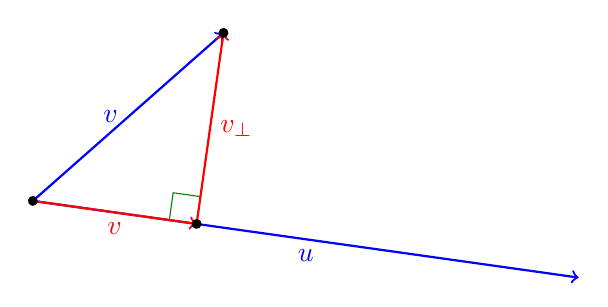
\begin{tikzpicture}[scale=0.7,rotate=-8]
      \draw[draw=green!50!black] (3,0.5) -- (2.5,0.5) -- (2.5,0);
      \draw[->, thick, blue](0,0) -- node[left]{$\vect{v}$} (3,3.5);
      \draw[->, thick, blue](0,0) -- node[below]{$\vect{u}$} (10,0);
      \draw[->, thick, red] (0,0) -- node[below]{$\vect{v}_{\coll}$} (3,0);
      \draw[->, thick, red] (3,0) -- node[right]{$\vect{v}_{\bot}$} (3,3.5);
      \draw[fill](0,0) circle [radius=2.25pt];
      \draw[fill](3,0) circle [radius=2.25pt];
      \draw[fill](3,3.5) circle [radius=2.25pt];
    \end{tikzpicture}
